\documentclass[12pt,t]{beamer}

%------------------------------------------------------------------------------
% configuration
%------------------------------------------------------------------------------
\RequirePackage{etex}
\usepackage{currfile-abspath}
\usepackage{../../themes/dbt}
\usepackage{catchfilebetweentags}

\setbeameroption{hide notes}
\setbeamertemplate{caption}{\raggedright\insertcaption\par}

\graphicspath{{images/}}
\getmainfile
\getabspath{\themainfile}
\let\mainabsdir\theabsdir
\let\mainabspath\theabspath

\newcommand{\insertcode}[2]{\lstinputlisting[label=samplecode, basicstyle=#1]{\mainabsdir/code/#2}}
\newcommand{\bi}{\begin{itemize}}
\newcommand{\ei}{\end{itemize}}
\newcommand{\ig}{\includegraphics}
\newcommand{\myhref}[1]{\href{#1}{\tt \scriptsize #1}}
\newcommand{\incnote}[1]{\note{\ExecuteMetaData[notes.tex]{#1}}}
\newcommand{\src}[2]{\vspace{-10pt}\caption{\href{#1}{\centering \tt \tiny [#2]}}}


%------------------------------------------------------------------------------
% title
%------------------------------------------------------------------------------
%------------------------------------------------------------------------------
% title
%------------------------------------------------------------------------------
% slide
\title{Systèmes d'exploitation pour l'embarqué}
\subtitle{UV 5.2 - Exécution et Concurrence}

\author{\href{}{Paul Blottière}}
\institute{
    \href{http://www.ensta-bretagne.fr/}{ENSTA Bretagne} \\[2pt]
    \href{}{\tt \scriptsize 2018 / 2019}
}
\date{
    \href{https://github.com/pblottiere}{\tt \scriptsize https://github.com/pblottiere} \\[2pt]
    %\href{blottiere.paul@gmail.com}{\tt \scriptsize blottiere.paul@gmail.com}
}

% info
\begin{document}

{
\setbeamertemplate{footline}{} % no page number here
\frame{
    \titlepage
} }

%------------------------------------------------------------------------------
% amélioration continue
%------------------------------------------------------------------------------
\begin{frame}{Amélioration continue}
    \subt{Contributions}
    \vspace{12pt}

    \begin{center}
    
\includegraphics[scale=0.7]{github.png}
    \end{center}

    \bi
    \itemsep12pt
    \item Dépôt du cours : \href{https://github.com/pblottiere/embsys}{\tt \scriptsize https://github.com/pblottiere/embsys}
    \item Souhaits d'amélioration, erreurs, idées de TP, ... : ouverture d'Issues
    \item Apports de corrections : Pull Request
    \ei
\end{frame}




%<**lecture_content>
%------------------------------------------------------------------------------
% lecture
%------------------------------------------------------------------------------
\begin{frame}[plain,c]
    \centering
    \huge\textcolor{title}{Les processus et les threads}
\end{frame}

%------------------------------------------------------------------------------
% plan
%------------------------------------------------------------------------------
\begin{frame}{Plan}
    \subt{}
    \vspace{10pt}

    \begin{enumerate}
        \itemsep12pt
        \item Définitions
        \item Outils
        \item Appels système
        \item Identification (PID, ...)
        \item Capacités d'un processus
        \item Création de processus
        \item Terminaison d'un processus
        \item Les pthreads
    \end{enumerate}

    \note {
    }
\end{frame}

%------------------------------------------------------------------------------
% def1
%------------------------------------------------------------------------------
\begin{frame}{Définitions (1)}
    \subt{Programme, Processus et Threads}
    \vspace{15pt}

    Programme : fichier exécutable, enregistré sur le disque
    \vspace{8pt}

    \onslide<2->{
        Processus :
        \bi
        \item programme en cours d'exécution
        \item disposent chacun d'un espace mémoire indépendant et protégé des autres
              processus (MMU)
        \item monothread ou multithread
        \ei
    }

    \onslide<3->{
        \vspace{8pt}
        Thread:
        \bi
        \item les threads d'un même processus partagent le même espace mémoire
        \item ne partagent pas les informations d'ordonnancement
        \ei
    }

    \incnote{def1}
\end{frame}

%------------------------------------------------------------------------------
% def2
%------------------------------------------------------------------------------
\begin{frame}{Définitions (2)}
    \subt{Ordonnanceur}

    \vspace{10pt}
    Linux est un kernel préemptif (capacité à exécuter ou stopper une tâche en
    cours) : imite un comportement multitâche.

    \onslide<2->{
        \vspace{10pt}
        L'ordonnanceur distribue le temps CPU entre les différents processus selon
        des politiques d'ordonnancement.

        \begin{figure}
            \centering
            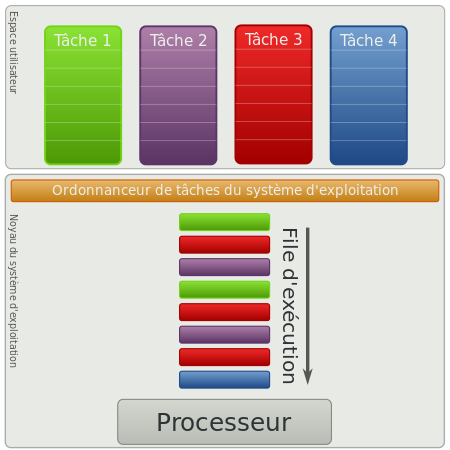
\includegraphics[scale=0.22]{ordonnanceur.png}
            \src{https://fr.wikipedia.org/wiki/Noyau_de_syst\%C3\%A8me_d\%27exploitation}{Exemple d'ordonnancement de tâches}
        \end{figure}
    }

    \incnote{def2}
\end{frame}

%------------------------------------------------------------------------------
% def3
%------------------------------------------------------------------------------
\begin{frame}{Définitions (3)}
    \subt{Ordonnanceur}

    \vspace{15pt}
    Il existe plusieurs politiques d'ordonnancement :
    \vspace{5pt}
    \bi
    \itemsep12pt
    \item FIFO (First In First Out) : file d'attente avec niveaux de
          priorité
    \item RR (Round Robin) : idem que FIFO mais avec en plus un
          quantum de temps (un processus dépassant ce quantum est mis
          en veille si une tâche ayant un même niveau de priorité
          est prête)
    \item OTHER : priorité dynamique recalculée en fonction de la
          priorité par défaut et du travail réalisé pendant le quantum
    \ei

    \incnote{def3}
\end{frame}

%------------------------------------------------------------------------------
% def4
%------------------------------------------------------------------------------
\begin{frame}{Définitions (4)}
    \subt{Process Control Block}

    \vspace{10pt}
    Un processus est représenté par un PCB (linux/sched.h).

    \onslide<2->{
        \vspace{10pt}
        Les éléments principaux de cette structure :
        \vspace{5pt}
        \bi
        \itemsep5pt
        \item run\_list : pointeur vers les processus suivants/précédents de la
              runqueue
        \item sibling : pointeurs vers les processus de même père
        \item sleep\_avg : temps moyen dans l'état Sleeping
        \item policy : OTHER, RR, FIFO
        \item pid : process identifier
        \item parent : process père
        \item children : liste des processus fils
        \ei
    }

    \incnote{def4}
\end{frame}

%------------------------------------------------------------------------------
% def5
%------------------------------------------------------------------------------
\begin{frame}{Définitions (5)}
    \subt{Les états}
    \vspace{15pt}

    \bi
    \itemsep12pt
    \item Running (R) : en cours d'exécution
    \item Sleeping (S) : non actif mais susceptible d'être réveillé par un
          évènement
    \item Stopped (T) : tâche temporairement arrêté. Attend un signal de
          redémarrage
    \item Zombie (Z) : tâche terminée mais code de retour non lu
    \ei

    \begin{figure}
        \centering
        
\includegraphics[scale=0.3]{state_tux.png}
    \end{figure}

\end{frame}

%------------------------------------------------------------------------------
% def6
%------------------------------------------------------------------------------
\begin{frame}{Définitions (6)}
    \subt{Les états}
    \vspace{8pt}

    \begin{figure}
        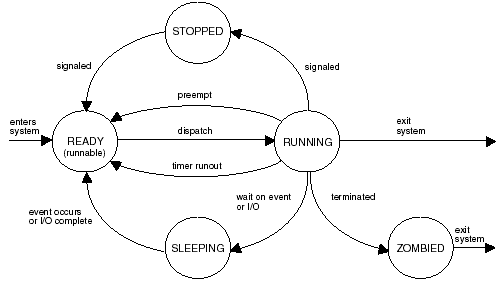
\includegraphics[scale=0.55]{state.png}
    \end{figure}

\end{frame}

%------------------------------------------------------------------------------
% def7
%------------------------------------------------------------------------------
\begin{frame}{Définitions (7)}
    \subt{Limites}
    \vspace{20pt}

    Un processus est évidemment limité en ressource!
    \vspace{10pt}

    \onslide<2->{
        Champ \textit{rlim} de la structure \textit{signals} du PCB :
        \vspace{8pt}
        \bi
        \itemsep12pt
        \item RLIMIT\_AS : taille max d'adressage (vérifiée lors d'un malloc)
        \item RLIMIT\_CORE : taille max du core dump
        \item RLIMIT\_CPU : temps CPU max en secondes
        \item ...
        \ei
    }

    \incnote{def7}
\end{frame}

%------------------------------------------------------------------------------
% analys1
%------------------------------------------------------------------------------
\begin{frame}{Outils (1)}
    \subt{Lister les processus en cours : commande ps}

    \vspace{-15pt}
    \begin{figure}
        \centering
        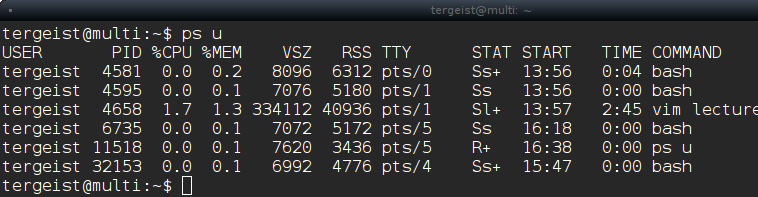
\includegraphics[scale=0.55]{ps_au.png}
    \end{figure}

    \onslide<2->{
        Les champs principaux :
        \bi
        \itemsep2pt
        \item USER : propriétaire du processus
        \item PID : numéro d'identification du processus
        \item CPU : pourcentage du temps CPU consacré
        \item MEM : mémoire totale utilisée par le processus
        \item STAT : code d'état du process
        \item TIME : temps CPU utilisé
        \item COMMAND : nom de la commande
        \ei
    }

    \incnote{analys1}
\end{frame}

%------------------------------------------------------------------------------
% analys2
%------------------------------------------------------------------------------
\begin{frame}{Outils (2)}
    \subt{Diverses commandes}

    \vspace{20pt}
    \bi
    \itemsep12pt
    \item nohup : ignore les déconnexion SIGHUP
    \item nice / renice : affectation de priorité (changement dans
          l'ordonnancement)
    \item kill / killall / pkill : terminaison de processus
    \item crontab : lancement programmé de processus
    \item cpulimit : limite le temps CPU d'un processus
    \ei

    \incnote{analys2}
\end{frame}

%------------------------------------------------------------------------------
% analys3
%------------------------------------------------------------------------------
\begin{frame}{Outils (3)}
    \subt{/proc}
    \vspace{10pt}

    {
        \textbf{/proc} est un système de fichier virtuel : les fichiers sont
        générés à la volée par le kernel!

        \onslide<2->{
            \vspace{10pt}
            \textbf{/proc} est une fenêtre sur le Kernel à travers laquelle on peut
            récupérer des informations sur le système et configurer certains
            comportements.

            \begin{figure}
                \centering
                
\includegraphics[scale=0.5]{fenetre-tux.png}
            \end{figure}
        }
    }

    \incnote{analys3}
\end{frame}

%------------------------------------------------------------------------------
% analys4
%------------------------------------------------------------------------------
\begin{frame}{Outils (4)}
    \subt{/proc}

    \vspace{3pt}
    Il existe un répertoire /proc/<PID> par processus qui contient toutes les
    informations le concernant :
    \bi
    \itemsep5pt
    \item cmdline : ligne de commande
    \item limits : limites des ressources
    \item mem : mémoire tenue par le processus
    \item d'autres : \myhref{http://man7.org/linux/man-pages/man5/proc.5.html}
    \ei

    \onslide<2->{
        \begin{figure}
            \centering
            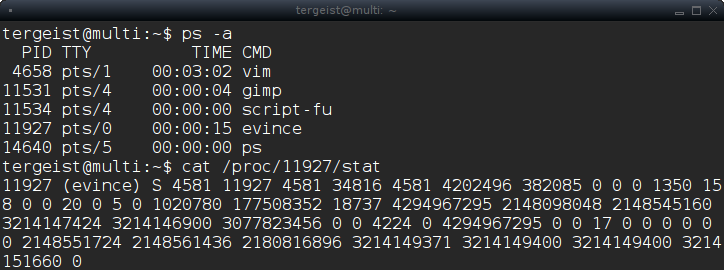
\includegraphics[scale=0.55]{proc_ex.png}
        \end{figure}
    }

    \incnote{analys4}
\end{frame}

%------------------------------------------------------------------------------
% syscall
%------------------------------------------------------------------------------
\begin{frame}{Appels Système}
    \subt{Qu'est-ce?}

    \vspace{15pt}
    Syscalls : Interface fondamentale entre le Kernel et les programmes de
    l'espace utilisateur et fournit via des wrappers de la libc.

    \onslide<2->{
        \vspace{15pt}
        Liste des appels système SUSv4 : \myhref{http://pubs.opengroup.org/onlinepubs/9699919799/}
    }

    \onslide<3->{
        \vspace{15pt}
        {
        Par exemple, \textit{unistd.h} est défini pour tous les UNIX et donne accès
        à des fonctions de l'API POSIX (read, write, fork, ...).
        }
    }

\end{frame}

%------------------------------------------------------------------------------
% ident1
%------------------------------------------------------------------------------
\begin{frame}{Identification (1)}
    \subt{PID et PPID}
    \vspace{15pt}

    Systèmes UNIX : règles précises concernant l'identification des utilisateurs
    et des processus!

    \onslide<2->{
        \vspace{10pt}
        Les appels système POSIX associés :
        \vspace{5pt}
        \bi
        \itemsep8pt
        \item pid\_t getpid (void) : entier 32 bits sous Linux. PID du processus
              courant.
        \item pid\_t getppid (void) : PID du père.
        \ei
    }

    \incnote{ident1}
\end{frame}

%------------------------------------------------------------------------------
% ident2
%------------------------------------------------------------------------------
\begin{frame}[fragile]{Identification (2)}
    \subt{PID et PPID (pid.c)}

    \insertcode{\footnotesize}{pid.c}

    \vspace{-20pt}
    \begin{figure}
        \centering
        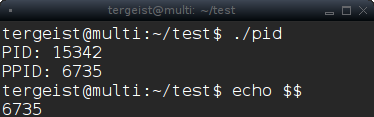
\includegraphics[scale=0.55]{pid.png}
    \end{figure}

    \incnote{ident2}
\end{frame}

%------------------------------------------------------------------------------
% ident3
%------------------------------------------------------------------------------
\begin{frame}{Identification (3)}
    \subt{UID}

    \vspace{5pt}
    Chaque processus s'exécute sous une identité propre. Il existe trois
    identifiants d'utilisateurs par processus :

    \bi
    \item UID réel : UID de l'utilisateur ayant lancé le programme
    \item UID effectif : indique les privilèges accordés au processus (flag
          setuid)
    \item UID sauvé : copie de l'ancien UID effectif lorsque celui-ci est modifié
          par le processus (automatique par le kernel)
    \ei

    \onslide<2->{
        \vspace{5pt}
        Les appels système associés :
        \bi
        \itemsep5pt
        \item POSIX : getuid / geteuid / setuid / setreuid
        \item Linux : setresuid
        \ei
    }

    \incnote{ident3}
\end{frame}

%------------------------------------------------------------------------------
% ident4
%------------------------------------------------------------------------------
\begin{frame}{Identification (4)}
    \subt{Groupe d'utilisateur, groupe de processus et groupe de groupe}

    \vspace{20pt}
    Il existe encore beaucoup de méthodes d'identification :
    \vspace{15pt}
    \bi
    \itemsep15pt
    \item par groupe d'utilisateurs du processus : GID
    \item par groupe de processus : PGID
    \item par session : SID
    \ei

    \incnote{ident4}
\end{frame}

%------------------------------------------------------------------------------
% capa1
%------------------------------------------------------------------------------
\begin{frame}{Capacités d'un processus}
    \subt{Privilèges}

    \vspace{15pt}
    Depuis la version 2.2 du Kernel Linux, chaque processus possède un jeu de
    capacités définissant précisément ses privilèges :

    \vspace{5pt}
    \bi
    \itemsep12pt
    \item CAP\_SYS\_BOOT : shutdown autorisé
    \item CAP\_SYS\_RAWIO : accès aux ports d'entrées / sorties
    \item d'autres : \myhref{http://manpagesfr.free.fr/man/man7/capabilities.7.html}
    \ei

    \onslide<2->{
        \vspace{15pt}
        Pour cela, utiliser la librairie libcap!
    }

    \incnote{capa1}
\end{frame}

%------------------------------------------------------------------------------
% crea1
%------------------------------------------------------------------------------
\begin{frame}{Création de processus (1)}
    \subt{fork}

    \vspace{15pt}
    {\textbf{fork}} est un appel système qui :
    \bi
    \itemsep8pt
    \item duplique le processus appelant (PID différent)
    \item les processus fils ne partagent pas le même espace mémoire que le père
    \item a un coût très faible en ressources (mécanisme COW [1])
    \ei

    \onslide<2->{
        \begin{figure}
            \centering
            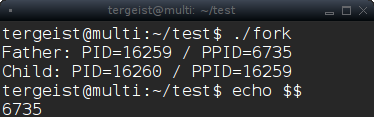
\includegraphics[scale=0.6]{fork.png}
        \end{figure}
    }

    \incnote{crea1}
\end{frame}

%------------------------------------------------------------------------------
% crea2
%------------------------------------------------------------------------------
\begin{frame}{Création de processus (2)}
    \subt{fork (fork.c)}

    \insertcode{\tiny}{fork.c}

\end{frame}

%------------------------------------------------------------------------------
% crea3
%------------------------------------------------------------------------------
\begin{frame}{Création de processus (3)}
    \subt{vfork}
    \vspace{10pt}

    {\textbf{vfork}} est un appel système qui :
    \bi
    \itemsep5pt
    \item créé un processus qui partage le même espace mémoire que le père
    \item bloque le père jusqu'à la terminaison du fils
    \ei

    \onslide<2->{
        \vspace{10pt}
        Peut créer des problèmes d'inversion de privilège car le fils n'est pas
        privilégié même si le père l'est : ne pas utiliser vfork!

        \vspace{15pt}
        => relevé dans un audit de sécurité de Linux en 2000!
    }

    \incnote{crea3}
\end{frame}

%------------------------------------------------------------------------------
% crea4
%------------------------------------------------------------------------------
\begin{frame}{Création de processus (4)}
    \subt{clone, execve, system, popen, ...}

    \vspace{20pt}
    Il existe de nombreux autres moyens d'initier un processus :
    \bi
    \itemsep12pt
    \item {\textbf{clone}} : paramétrage précis du comportement du fils
    \item {\textbf{execve}} : espace mémoire totalement remplacé
    \item {\textbf{system}} : exécute une commande shell (à bannir bien sûr...)
    \item {\textbf{popen / pclose}} : pipe + fork + invocation dans le shell (idem)
    \ei

    \incnote{crea4}
\end{frame}

%------------------------------------------------------------------------------
% init1
%------------------------------------------------------------------------------
%\begin{frame}{Phase d'init (1)}
%    \subt{Kernel Thread}
%    \incnote{init1}
%\end{frame}

%------------------------------------------------------------------------------
% init2
%------------------------------------------------------------------------------
%\begin{frame}{Phase d'init (2)}
%    \subt{init}
%    \incnote{init2}
%\end{frame}

%------------------------------------------------------------------------------
% init3
%------------------------------------------------------------------------------
%\begin{frame}{Phase d'init (3)}
%    \subt{init toujours en vie...}
%    \incnote{init3}
%\end{frame}

%------------------------------------------------------------------------------
% end1
%------------------------------------------------------------------------------
\begin{frame}{Terminaison d'un processus (1)}
    \subt{Généralité}

    \vspace{5pt}
    Un processus peut se terminer :
    \bi
    \item volontairement : tâche terminée, erreur gérée, ...
    \item involontairement : erreur non gérée, Ctrl-C, ...
    \ei

    \onslide<2->{
        \vspace{5pt}
        Un processus retourne un code d'erreur. Pour être portable :
        \bi
        \item un main doit toujours retourner un {\textbf{int}}!
        \item utiliser EXIT\_SUCCESS et EXIT\_FAILURE
        \ei
    }

    \onslide<3-> {
        \vspace{5pt}
        Ce code d'erreur est ensuite lu par le père :

        \begin{figure}
            \centering
            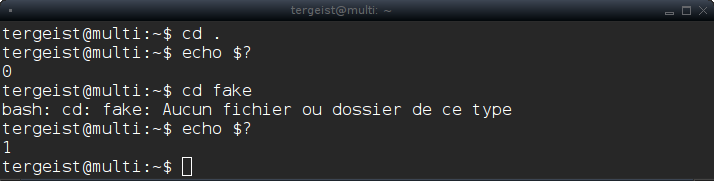
\includegraphics[scale=0.55]{code_retour.png}
        \end{figure}
    }

    \incnote{end1}
\end{frame}

%------------------------------------------------------------------------------
% end2
%------------------------------------------------------------------------------
\begin{frame}{Terminaison d'un processus (2)}
    \subt{Je vais bien, tout va bien...}

    \vspace{10pt}
    Pour une terminaison normale, plusieurs appels système :
    \bi
    \item {\textbf{exit}} : termine le programme avec un code de retour.
    \item {\textbf{atexit}} : permet de spécifier des fonctions à appeler en
          fin d'exécution
    \item {\textbf{on\_exit}} : comme atexit mais beaucoup moins standard (pas
          sur OSX) donc préférer atexit
    \ei

    \onslide<2->{
        \vspace{10pt}
        File d'exécution de {\textbf{exit}} :
        \begin{enumerate}
        \itemsep8pt
        \item exécute les fonctions enregistrées par atexit / on\_exit
        \item ferme les flux d'entrées / sorties
        \item appel \_exit qui termine le processus et retourne le code d'erreur
        \end{enumerate}
    }

    \incnote{end2}
\end{frame}

%------------------------------------------------------------------------------
% end3
%------------------------------------------------------------------------------
\defverbatim{\lstulimit}{
    \begin{lstlisting}
> ulimit -c unlimited
    \end{lstlisting}
}

\defverbatim{\lstcore}{
    \begin{lstlisting}
> cat /proc/sys/kernel/core_pattern
core
    \end{lstlisting}
}

\begin{frame}[fragile]{Terminaison d'un processus (3)}
    \subt{Terminaison anormale}

    \vspace{10pt}
    Lors d'une terminaison anormale, un fichier core est généré.

    \vspace{10pt}
    Ce fichier est une image mémoire de l'instant de l'anomalie permettant de
    rejouer le scénario (avec gdb)!

    \onslide<2->{
        \vspace{10pt}
        On peut modifier le pattern de création du fichier core!
        \vspace{5pt}
        \lstcore
    }

    \onslide<3->{
        \vspace{10pt}
        Pour créer des fichiers core sans limite de taille :
        \vspace{5pt}
        \lstulimit
    }

    \incnote{end3}
\end{frame}

%------------------------------------------------------------------------------
% end4
%------------------------------------------------------------------------------
\begin{frame}{Terminaison d'un processus (4)}
    \subt{Signaux}

    \vspace{10pt}
    Un processus peut aussi se terminer lors de la réception d'un signal :
    \bi
    \item Ctrl-Alt gr-\textbackslash : SIGQUIT
    \item Ctrl-C : SIGINT
    \item kill / pkill : SIGKILL
    \item beaucoup d'autres, dont certains définis par les normes POSIX temps réel
    \ei

    \onslide<2->{
        \vspace{10pt}
        Pour fermer proprement une application, il est indispensable de gérer
        l'interception des signaux!

        \begin{figure}
            \centering
            
\includegraphics[scale=0.25]{tux_propre.png}
        \end{figure}
    }

    \incnote{end4}
\end{frame}

%------------------------------------------------------------------------------
% end5
%------------------------------------------------------------------------------
\begin{frame}{Terminaison d'un processus (5)}
    \subt{Signaux (signals.c)}

    \begin{figure}
        \centering
        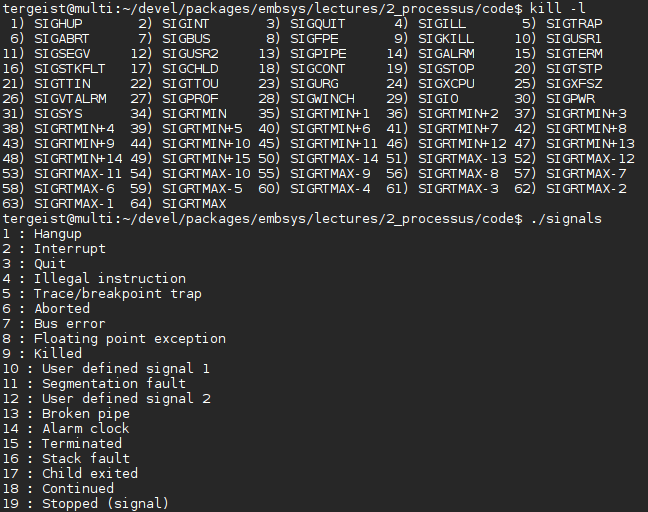
\includegraphics[scale=0.55]{signals.png}
    \end{figure}

    \incnote{end5}
\end{frame}

%------------------------------------------------------------------------------
% end6
%------------------------------------------------------------------------------
\begin{frame}{Terminaison d'un processus (6)}
    \subt{Signaux}

    \vspace{10pt}
    Pour gérer les signaux, deux méthodes :
    \vspace{10pt}
    \bi
    \itemsep8pt
    \item {\textbf{signal}} : très simple, défini par Ansi C et SUSv4 mais peut
          avoir des problèmes de portabilité entre systèmes UNIX
    \item {\textbf{sigaction}} : plus complexe mais complètement portable!
    \ei

    \onslide<2->{
        \begin{figure}
            \centering
            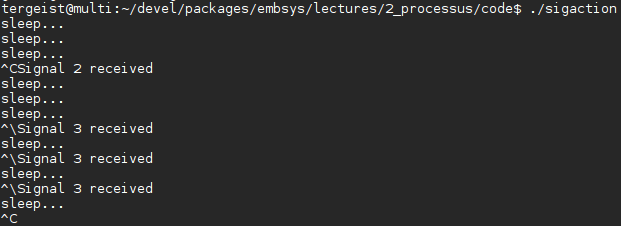
\includegraphics[scale=0.55]{sigaction.png}
        \end{figure}
    }

    \incnote{end6}
\end{frame}

%------------------------------------------------------------------------------
% end7
%------------------------------------------------------------------------------
\begin{frame}{Terminaison d'un processus (7)}
    \subt{Signaux (sigaction.c)}

    \insertcode{\tiny}{sigaction.c}

    \incnote{end7}
\end{frame}

%------------------------------------------------------------------------------
% pthread1
%------------------------------------------------------------------------------
\begin{frame}{Les pthreads (1)}
    \subt{Processeur, coeur et cache}

    \vspace{10pt}
    Instructions simultanées:
    \bi
    \itemsep8pt
    \item CPU single-core: 1 seule instruction
    \item CPU multi-core: 1 instruction par core
    \ei

    \onslide<2->{
        \vspace{10pt}
        Mémoire cache d'un CPU:
        \bi
        \itemsep6pt
        \item L1: + rapide / - gros
        \item L2: - rapide / + gros
        \item L3: -- rapide / ++ gros
        \ei
    }

\end{frame}

%------------------------------------------------------------------------------
% pthread1
%------------------------------------------------------------------------------
\begin{frame}{Les pthreads (1)}
    \subt{Processeur, coeur et cache}

    \vspace{10pt}
    Architectures dépendantes en fonction des processeurs.

    \onslide<2->{
        \vspace{10pt}
        Par exemple:
        \begin{figure}
            \centering
            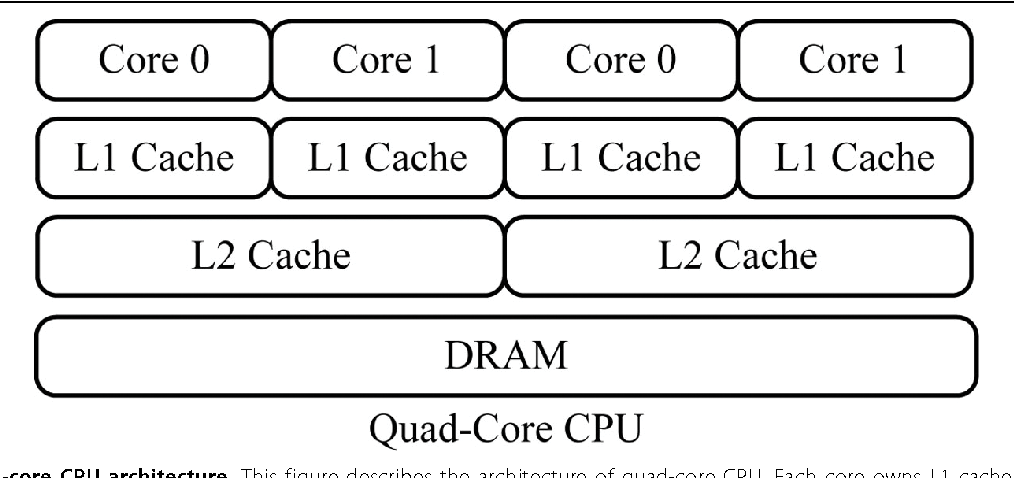
\includegraphics[scale=0.25]{core.png}
        \end{figure}
    }

\end{frame}

%------------------------------------------------------------------------------
% pthread1
%------------------------------------------------------------------------------
\begin{frame}{Les pthreads (1)}
    \subt{Multi Processing, Multi Threading, Hyper Threading}

    \vspace{8pt}
    Multi Processing:
    \bi
    \itemsep4pt
    \item Concept logiciel: espace mémoire dédié, ...
    \item Un process peut tourner sur 1 core
    \ei

    \onslide<2->{
        \vspace{8pt}
        Multi Threading:
        \bi
        \itemsep4pt
        \item Concept logiciel: espace mémoire partagé, ...
        \item Un process peut contenir plusieurs threads, donc 1 core peut gérer plusieurs threads
        \ei
    }

    \onslide<3->{
        \vspace{8pt}
        Hyper Threading:
        \bi
        \itemsep4pt
        \item Concept matériel: technologie créée par Intel
        \item Gestion plus efficace de plusieurs threads par 1 seul core
        \item Notion de core logique (1 core -> 2 core logiques)
        \ei
    }
\end{frame}

%------------------------------------------------------------------------------
% pthread1
%------------------------------------------------------------------------------
\begin{frame}{Les pthreads (1)}
    \subt{Présentation}

    \vspace{15pt}
    \begin{figure}
        \centering
        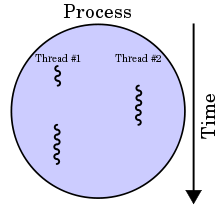
\includegraphics[scale=0.4]{thread.png}
    \end{figure}

    \vspace{15pt}
    Threads avec portabilité SUSv4 sous Linux : les pthreads!

    \incnote{pthread1}
\end{frame}

%------------------------------------------------------------------------------
% pthread2
%------------------------------------------------------------------------------
\begin{frame}{Les pthreads (2)}
    \subt{NTPL}

    \vspace{20pt}
    Les pthreads sont intégrés dans le Kernel Linux depuis la version 2.6 via
    la bibliothèque Native Posix Thread Library (NTPL).

    \onslide<2->{
        \vspace{20pt}
        Pour utiliser les threads de la NTPL :
        \bi
        \item \#include <pthread.h>
        \item gcc -pthread
        \ei
    }

    \incnote{pthread2}
\end{frame}

%------------------------------------------------------------------------------
% pthread3
%------------------------------------------------------------------------------
\begin{frame}[fragile]{Les pthreads (3)}
    \subt{Création et identification}
    \vspace{10pt}

    Identifiant :
    \bi
    \itemsep8pt
    \item d'un processus : pid\_t
    \item d'un thread : pthread\_t
    \ei

    \vspace{10pt}
    Pour la création d'un pthread :
    \vspace{5pt}
    %\lstcreate
    \begin{lstlisting}
int pthread_create(pthread_t * thread,
                   pthread_attr_t * attributes,
                   void * (* funct) (void * arg),
                   void * argument)
    \end{lstlisting}

    \onslide<2->{
        \vspace{10pt}
        \begin{figure}
            \centering
            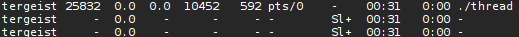
\includegraphics[scale=0.7]{thread2.png}
        \end{figure}
    }

    \incnote{pthread3}
\end{frame}

%------------------------------------------------------------------------------
% pthread4
%------------------------------------------------------------------------------
\begin{frame}{Les pthreads (4)}
    \subt{Application (thread.c)}

    \insertcode{\tiny}{thread.c}

    \incnote{pthread4}
\end{frame}

%------------------------------------------------------------------------------
% pthread5
%------------------------------------------------------------------------------
\begin{frame}{Les pthreads (5)}
    \subt{Terminaison}

    \vspace{15pt}
    Cas où tout le processus (et donc tous les threads) est tué :
    \bi
    \itemsep12pt
    \item le thread principal fait appel à {\textbf{return}} dans le main
    \item le thread principal fait appel à {\textbf{exit}}
    \item un des threads fait appel à {\textbf{exit}}
    \item un des threads se termine involontairement
    \ei

    \onslide<2->{
        \vspace{15pt}
        Cas où juste un threads est tué :
        \bi
        \item le thread fait appel à la fonction {\textbf{pthread\_exit}}
        \ei
    }

    \incnote{pthread5}
\end{frame}

%------------------------------------------------------------------------------
% pthread6
%------------------------------------------------------------------------------
\begin{frame}{Les pthreads (6)}
    \subt{join}

    \vspace{15pt}
    Un pthread stocke sa valeur de retour dans la pile.

    \vspace{15pt}
    Pour récupérer la valeur de retour, il faut utiliser {\textbf{pthread\_join}}.
    Cependant, le thread appelant bloque jusqu'à la fin du thread!

    \onslide<2-> {
        \vspace{15pt}
        Un processus a un espace mémoire limité donc ???
    }

    \vspace{15pt}
    \onslide<3-> {
        => comme un thread stocke sa valeur de retour dans la pile, un processus
        peut instancier seulement un nombre limité de thread!
    }

    \incnote{pthread6}
\end{frame}

%------------------------------------------------------------------------------
% pthread7
%------------------------------------------------------------------------------
\begin{frame}{Les pthreads (7)}
    \subt{Nombre maximum de threads (maxthread.c)}

    \insertcode{\tiny}{maxthread.c}

    \begin{figure}
        \centering
        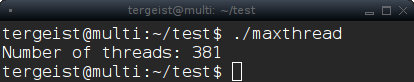
\includegraphics[scale=0.55]{maxthread.png}
    \end{figure}

    \incnote{pthread7}
\end{frame}

%------------------------------------------------------------------------------
% pthread8
%------------------------------------------------------------------------------
\begin{frame}{Les pthreads (8)}
    \subt{detach (unlthread.c)}

    \vspace{20pt}
    Pour indiquer au kernel de ne pas stocker les valeurs de retours dans la pile,
    on peut utiliser {\textbf{pthread\_detach}}.

    \onslide<2->{
        \vspace{20pt}
        => un processus peut alors créer un nombre illimité de thread!

        \begin{figure}
            \centering
            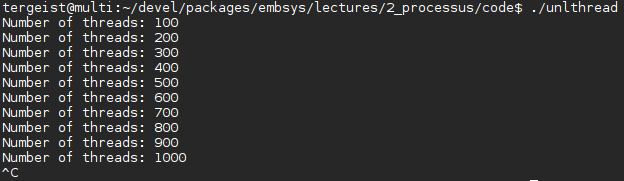
\includegraphics[scale=0.6]{unlthread.png}
        \end{figure}
    }

    \incnote{pthread8}
\end{frame}

%------------------------------------------------------------------------------
% pthread9
%------------------------------------------------------------------------------
\begin{frame}{Les pthreads (9)}
    \subt{Thread Safety et \_REENTRANT}

    \vspace{10pt}
    Un code Thread Safe peut travailler {\textbf{correctement}} en mode
    multitâches, c'est à dire être utilisé simultanément par plusieurs threads
    au sein d'un même espace mémoire.

    \onslide<2-> {
        \vspace{10pt}
        L'option -D\_REENTRANT indique au compilateur que les fonctions peuvent
        être utilisées simultanément (évite la duplication en RAM).

        \begin{figure}
            \centering
            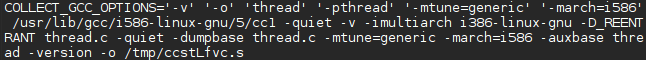
\includegraphics[scale=0.6]{reent.png}
        \end{figure}
    }

    \onslide<3-> {
            Une fonction réentrante n'est pas forcément Thread Safe. \\
            => des mécanismes d'exclusion mutuelle sont nécessaires dû au
            caractère préemptif du Kernel!
    }

    \incnote{pthread9}
\end{frame}

%------------------------------------------------------------------------------
% pthread10
%------------------------------------------------------------------------------
\begin{frame}{Les pthreads (10)}
    \subt{Synchronisation}

    \vspace{15pt}
    Utilisation de {\textbf{mutex}} (mutual exclusion) pour la synchronisation
    d'accès à des données partagées.

    \onslide<2-> {
        \vspace{15pt}
        Les mutex sont des verrous à deux états (libre ou verrouillé) et
        représentés par des variables de type {\textbf{pthread\_mutex\_t}}.

        \begin{figure}
            \centering
            
\includegraphics[scale=0.25]{mutex.jpg}
        \end{figure}
    }

    \incnote{pthread10}
\end{frame}

%------------------------------------------------------------------------------
% pthread11
%------------------------------------------------------------------------------
\begin{frame}{Les pthreads (11)}
    \subt{Mutex et RW Lock}

    \vspace{5pt}
    Mutex avec type {\textbf{pthread\_mutex\_t}} :
    \bi
    \item création statique : PTHREAD\_MUTEX\_INITIALIZER
    \item création dynamique : {\textbf{pthread\_mutex\_init}}
    \item libération de la variable : {\textbf{pthread\_mutex\_destroy}}
    \item verrouillage : {\textbf{pthread\_mutex\_lock}}
    \item déverrouillage : {\textbf{pthread\_mutex\_unlock}}
    \ei

    \onslide<2-> {
        \vspace{5pt}
        RW Lock avec type {\textbf{pthread\_rwlock\_t}} :
        \bi
        \item création statique : PTHREAD\_RWLOCK\_INITIALIZER
        \item création dynamique : {\textbf{pthread\_rwlock\_init}}
        \item libération de la variable : {\textbf{pthread\_rwlock\_destroy}}
        \item demande Read Only : {\textbf{pthread\_rwlock\_rdlock}}
        \item demande RW : {\textbf{pthread\_rwlock\_wrlock}}
        \item déverrouillage : {\textbf{pthread\_rwlock\_unlock}}
        \ei
    }

    \incnote{pthread11}
\end{frame}

%------------------------------------------------------------------------------
% pthread12
%------------------------------------------------------------------------------
\begin{frame}{Les pthreads (12)}
    \subt{Programmation avancée}

    \vspace{15pt}
    Les applications concurrentes sont complexes à mettre en place et de très
    nombreuses fonctions existent pour gérer de manière précise le comportement
    d'un thread :

    \vspace{10pt}
    \onslide<2->{
        \bi
        \itemsep12pt
        \item nettoyage : pthread\_cleanup\_push, pthread\_cleanup\_pop
        \item taille de la pile : pthread\_attr\_getstackaddr, pthread\_attr\_setstackaddr
        \item variable globale à portée d'un seul thread : pthread\_key\_create
        \item et encore beaucoup d'autres...
        \ei
    }

    \incnote{pthread12}
\end{frame}

%------------------------------------------------------------------------------
% conclusion
%------------------------------------------------------------------------------
\begin{frame}{Conclusion}

    \centering
    \vspace{20pt}
    \LARGE{
    Il faut être un vieux sage pour maîtriser tous les aspects de la
    programmation multithread!
    }

    \begin{figure}
        \centering
        
\includegraphics[scale=0.35]{sage.png}
    \end{figure}

\end{frame}

%------------------------------------------------------------------------------
% ref
%------------------------------------------------------------------------------
\begin{frame}{Références}
    \vspace{30pt}

    \bi
    \itemsep12pt
    \item Linux Embarqué - Pierre Ficheux
    \item Développement système sous Linux - Christophe Blaess
    \item Modern Operating Systems - Andrew Tanenbaum
    \item [1] http://www.eastrivervillage.com/The-Linux-COW/
    \ei
\end{frame}
%<//lecture_content>

\end{document}
